%==============================================================================
\chapter{SURVEY}\label{sec:5}
%==============================================================================

%==============================================================================
% Neste capítulo informações mais detalhadas são apresentadas sobre o levantamento (\textit{survey}) que foi conduzido. 
% Na \Cref{sec:survey-protocol}, é apresentado detalhes sobre o protocolo adotado, autor de referencia e divisão de tarefas entre os pesquisadores. 
% Logo na \Cref{sec:survey-threats}, as ameaças a validade do estudo são relatadas, e por fim na \Cref{sec:survey-results}, todos os resultados alcançados durante a execução são discorridos.

In this chapter, more detailed information is presented about the survey that was conducted.
The survey was a collaborative effort between two authors, just like the grey literature systematic review discussed in the preceding chapter. Later, we'll go over each person's responsibilities.
In \Cref{sec:survey-protocol}, details about the adopted protocol, reference author, and task division among researchers are presented.
The \Cref{sec:survey-threats}, reports threats to the validity of the study, and finally, in \Cref{sec:survey-results}, all results achieved during execution are discussed.
%==============================================================================

\section{Survey Protocol} \label{sec:survey-protocol}

%==============================================================================
% Um levantamento (\textit{survey}) é uma abordagem de coleta e análise de dados em que os participantes respondem a perguntas ou a declarações que foram desenvolvidas antecipadamente. 
% O protocolo escolhido para a elaboração desta pesquisa foi inspirado nas diretrizes propostas por \textcite{kasunic2005designing}, em \textit{Designing an effective survey} e está ilustrado na \Cref{fig:setepassos}.

According to \textcite{kasunic2005designing}, a survey is a method of gathering and analyzing data in which participants respond to pre-formulated questions or statements. The guidelines suggested by the author served as inspiration for the protocol that was developed for this study and is shown in \Cref{fig:setepassos}.

%==============================================================================

\begin{figure}[htb]
  \caption{Seven steps of the research process}\label{fig:setepassos}
  \begin{center}
    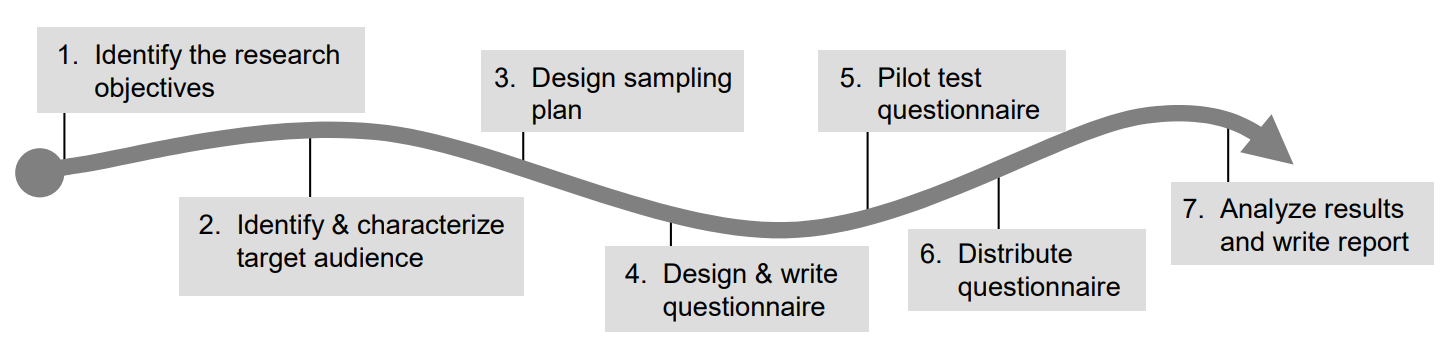
\includegraphics[width=16cm]{img/5-kasunic-process.png}
  \end{center}
  \fonte{\cite{kasunic2005designing}.}
\end{figure}

%==============================================================================
% Como será dito posteriormente, o objetivo é compreender as necessidades de discentes e docentes em relação aos projetos e atividades de extensão. 
% A escolha do \textit{survey} como abordagem de coleta de dados se deve ao fato de que as características de uma pesquisa deste tipo nos permite generalizar sobre as crenças e opiniões de muitas pessoas estudando apenas um subconjunto delas \cite{kasunic2005designing}. 
% Sendo, neste caso, a ferramenta ideal.

The goal is to comprehend teacher and student needs with regard to outreach projects and activities, as will be stated later.
The choice of \textit{survey} as a data collection approach is due to the fact that the characteristics of a survey of this type allow us to generalize about the beliefs and opinions of many people by studying only a subset of them \cite{kasunic2005designing}.
In this case, the ideal tool.
%==============================================================================

%==============================================================================
% Tendo em vista que esta pesquisa foi executada por dois estudantes, a carga de trabalho foi dividida, de maneira que a qualidade e desempenho fossem melhorados. 
% Na \Cref{tbl:survey-tasks} se encontra a divisão de atividades adotada, contemplando as já definidas por \textcite{kasunic2005designing}.

Due to the fact that this research was conducted by two students, efficiency and effectiveness were enhanced by dividing the workload.
\Cref{tbl:survey-tasks} shows the division of adopted activities, taking into account those that \textcite{kasunic2005designing} has already defined.
%==============================================================================

% Tabela \Cref{tbl:survey-tasks} Activity Division
\begin{table}[!htb]
  \centering
  \caption{Tasks Separation}
  \label{tbl:survey-tasks}
  \footnotesize
  \begin{tabular}{l|l}
    \bottomrule
    \rowcolor[rgb]{0.753,0.753,0.753} \multicolumn{1}{c|}{\textbf{Activity}}                             & \multicolumn{1}{c}{\textbf{Responsibility}} \\
    \hline
    \rowcolor[rgb]{0.898,0.898,0.898} Define and document research objectives                            & Lucas F.                                    \\
    Define and document research questions                                                               & Lucas F.                                    \\
    \rowcolor[rgb]{0.898,0.898,0.898} Define and document how research results will be used              & Lucas F.                                    \\
    Define the appropriate target audience for the research                                              & Igor C.                                     \\
    \rowcolor[rgb]{0.898,0.898,0.898} Determine the appropriate media to apply the research in           & Igor C.                                     \\
    Recruit members of the target audience to participate in pilot test                                  & Igor C.                                     \\
    \rowcolor[rgb]{0.898,0.898,0.898} Breakdown research questions into questionnaire topics             & Lucas F.                                    \\
    Organize and sequence questions                                                                      & Lucas F.                                    \\
    \rowcolor[rgb]{0.898,0.898,0.898} Review the questionnaire based on the pilot test                   & Igor C. and Lucas F.                        \\
    Perform the pilot test                                                                               & Igor C. and Lucas F.                        \\
    \rowcolor[rgb]{0.898,0.898,0.898} Evaluate comments                                                  & Igor C. and Lucas F.                        \\
    Perform final corrections before the distribution of the questionnaire                               & Lucas F.                                    \\
    \rowcolor[rgb]{0.753,0.753,0.753} \multicolumn{1}{c|}{\textbf{Questionnaire ready for distribution}} &                                             \\
    Distribute questionnaires                                                                            & Lucas F.                                    \\
    \rowcolor[rgb]{0.898,0.898,0.898} Monitor answers                                                    & Igor C. and Lucas F.                        \\
    Send reminders                                                                                       & Igor C.                                     \\
    \rowcolor[rgb]{0.753,0.753,0.753} \multicolumn{1}{c|}{\textbf{Questionnaire response deadline}}      &                                             \\
    Perform analysis                                                                                     & Igor C. and Lucas F.                        \\
    \rowcolor[rgb]{0.898,0.898,0.898} Write draft report                                                 & Igor C.                                     \\
    Revise draft                                                                                         & Igor C. and Lucas F.                        \\
    \rowcolor[rgb]{0.898,0.898,0.898} Perform the final corrections                                      & Igor C. and Lucas F.                        \\
    \toprule
  \end{tabular}
\end{table}

\subsection{Identify the Research Objectives} \label{sec:survey-objectives}
% Objetivo do survey -> refinamento dos requisitos, validar, importancia
% Transformar em uma questão de pesquisa, pergunta
% grey gerou resultados pra usar no survey com o olhar dos futuros usuarios

%==============================================================================
% O objetivo deste primeiro passo é identificar qual a importância e o por que de fazer um survey, o que poderia ser conquistado com ele.
% Levando em conta os resultados gerados pela revisão na literatura cinza, mencionados no \Cref{grey_literature}, foi possível elaborar questões de maneira que o participante informe, na sua visão, a importância de determinado requisito levantado. 
% Logo, o objetivo deste survey é ordená-los por prioridade, utilizando a opinião de possíveis usuários finais.

This first step's goal is to explain why conducting a survey is important and what can be accomplished by doing so.
Taking into account the results generated by the review in the gray literature, mentioned in \Cref{grey_literature}, it was possible to elaborate questions in a way that the participant informs, in his view, the importance of a certain requirement raised.
As a result, the goal of this survey is to prioritize them based on the views of potential end users.
%==============================================================================

%==============================================================================
% Além de ser perguntado a opinião dos participantes, foi permitido com que eles fornecessem sugestões ou melhorias em relação a requisitos da ferramenta, já que um dos objetivos da pesquisa está voltado a entender as necessidades dos possíveis usuários do sistema. 
% Assim, tendo uma base mais sólida para começar o processo de desenvolvimento da solução, com os escopos das atividades mais bem definidos.

In addition to being asked their opinions, participants were free to offer suggestions or improvements in relation to the needs of the tool, as one of the study's goals is to identify the needs of potential system users.
Consequently, with a more solid foundation and a more clearly defined scope of activities, the solution development process will begin.
%==============================================================================
\subsection{Identify and Characterize the Target Audience} \label{sec:survey-targets}
%==============================================================================
% Neste estágio, é necessário olhar para os possíveis públicos respondentes e identificar quem será o público respondente e quem é a população do estudo. 
% Assim sendo, a população é composta por todos as pessoas dentro da comunidade acadêmica, logo foi escolhido para representarem a amostra desta população os coordenadores de programas ou projetos de extensão, docentes e discentes, tendo preferência em participantes que tenham experiência com atividades de extensão. 
% Com este público é possível ter o ponto de vista de todos os usuários da ferramenta, quem cria atividades e quem se inscreve em uma.

At this stage, it is necessary to look at the possible respondent audiences and identify who will be the respondent audience and who the study population is.
Therefore, the population is made up of all people within the academic community, so the coordinators of outreach programs or projects, professors and students were chosen to represent the sample of this population, with preference given to participants who have experience with outreach activities.
With this audience, it is possible to understand all tool users' perspectives, including those of activity creators and subscribers.
%==============================================================================
% Para possívelmente conseguir melhores sugestões nas respostas do survey, foi necessário abrangir a maior quantidade de campus da \ac{UNIPAMPA} possivel, era esperado que campus como Uruguaiana, Bagé e Dom Pedrito que, como visto na \Cref{fig:number-of-projects} foram os campus que mais possuiram atividades de extensão no ano de 2017 de acordo com \cite{relatorio-2017}, fornecessem mais respondentes, mas no final isto nao aconteceu.

% \begin{figure}[htb]
%   \caption{Number of Projects Contemplated in the Internal Public Notices}\label{fig:number-of-projects}
%   \begin{center}
%     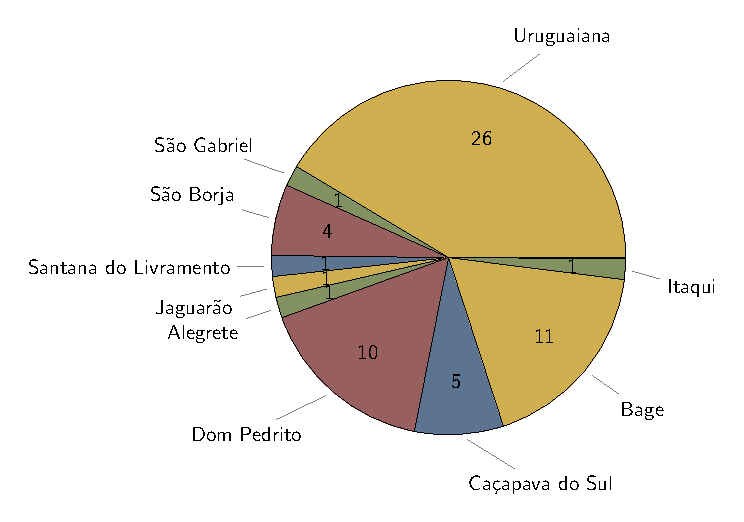
\includegraphics[width=16cm]{img/uruguaiana.pdf}
%   \end{center}
%   \fonte{Adapted from \cite{relatorio-2017}}
% \end{figure}

\subsection{Design the Sampling Plan} \label{sec:survey-sampling}

%==============================================================================
% De acordo com \textcite{kasunic2005designing}, o objetivo desta fase é determinar os seguintes tópicos:
% \begin{itemize}
%     \item How individuals will be selected to participate in the survey;
%     \item The required size of the sample.
% \end{itemize}

According to \textcite{kasunic2005designing}, the objective of this phase is to determine the following topics:
\begin{itemize}
    \item How individuals will be selected to participate in the survey;
    \item The required size of the sample.
\end{itemize}
%==============================================================================

%==============================================================================
% Por isso, o primeiro tópico buscou abrangir a maioria de campus da \ac{UNIPAMPA} possível por meio de envio de emails para as suas secretarias academicas, direcionados para os alunos e para listas de coordenadores de programas e projetos de extensão, mantendo o equilibrio entre docentes e discentes. 
% Com isso, campus como Uruguaiana e Bagé que, como visto na \Cref{fig:number-of-projects} foram os campus que mais executaram atividades de extensão no ano de 2021 \cite{relatorio-2021}, assim, esperava-se que fornecessem mais respondentes para a pesquisa.

Therefore, the first topic sought to cover as many \ac{UNIPAMPA} campuses as possible by sending emails to its Academic Secretariats, directed to students and to lists of coordinators of programs and outreach projects, keeping the balance between teachers and students.
As a result, it was anticipated that campuses like Uruguaiana and Bagé, which can be seen in \Cref{fig:number-of-projects} as being the campuses that performed outreach activities the most in 2021 \cite{relatorio-2021}, would contribute more respondents to the survey.
%==============================================================================

\begin{figure}[htb]
  \caption{Number of Projects Contemplated in the Internal Public Notices}\label{fig:number-of-projects}
  \begin{center}
    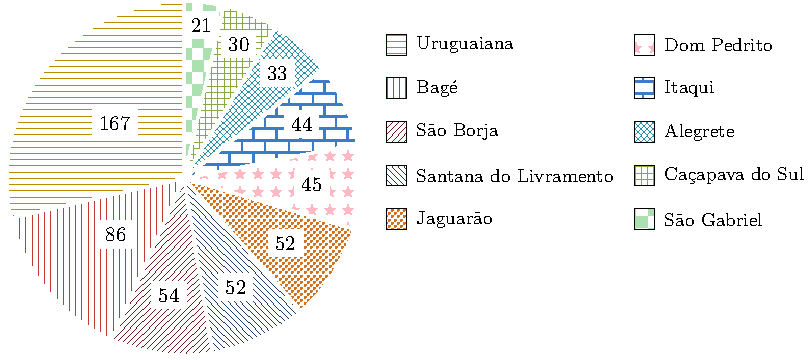
\includegraphics[width=.9\textwidth]{img/5-number-of-projects.pdf}
  \end{center}
  \fonte{Adapted from \cite{relatorio-2021}}
\end{figure}

%==============================================================================
% Em relaçao ao tamanho mínimo da amostra, tamanhos entre 100 e 150 respondentes já seriam suficientes, pois além das respostas quantitativas teriam todas as respostas qualitativas com sugestões e melhorias, demandando mais tempo para análise.

Along with all of the quantitative responses, each respondent had the chance to discuss the questions in greater detail, allowing for qualitative feedback. This added significantly to the amount of work needed to conduct the analysis. The questionnaire received 123 responses in total.
%==============================================================================

%==============================================================================
% A separação da amostra é um ponto essencial para a melhor eficiência do survey, estando de acordo com a prática recomendada 22 definida por \textcite{Jefferson}, em que diz que a amostra deve ser dividida de acordo com as suas caracteristicas e semelhanças. 
% Para contemplá-la, os respondentes do questionário que se declarassem como \acp{TAE} ou docentes eram direcionados para uma área do questionário, e discentes para outra, ambas as áreas com perguntas relacionadas ao perfil reclarado pelo respondente.

The separation of the sample is an essential point for the best efficiency of the survey, being in accordance with the recommended practice 22 defined by \textcite{Jefferson}, which says that the sample should be divided according to its characteristics and similarities.
To contemplate it, the questionnaire respondents who declared themselves as \acp{ATE} or professors were directed to one area of the questionnaire, and students to another, both areas with questions related to the profile claimed by the respondent.
%==============================================================================
\subsection{Design and Write the Questionnaire} \label{sec:survey-questionnaire}

% (kasunic) objetivos e caracteristicas da sample para fazer o questionario, importancia dos dois
% (guideline) resultados dependem da qualidade das perguntas

% (kasunic) 4 tipos de perguntas, colcoar as que se encaixam em cada uma
% (kasunic) close ended e open ended questions 52, todas sao ordinal responses usando MoSCoW

% Colocar o questionario em apendice
%==============================================================================
% \textcite{kasunic2005designing} ressalta que para a estruturação e escrita do questionário, os objetivos de pesquisa e as características da amostra devem ser levados em conta. 
% De acordo com o autor, questionarios que não possuem objetivos bem definidos tem mais chances de possuirem perguntas que só consomem tempo do respondente, ele ressalta isso com uma pergunta \textcite[p.34]{kasunic2005designing} ``How can you reach insightful conclusions if you do not know what you were looking for or planning to observe?'', neste questionário o objetivo é bem definido, focado em priorização de requisitos e levantamento de sugestões pelos possíveis usuários finais como bem descrito na \Cref{sec:survey-objectives}. 
% Da mesma maneira, as caracteristicas da amostra são importantes para escrever as perguntas de um modo que todos entendam e não apenas pensando no entendimento dos proprios pesquisadores. 
% % \textcite[p.23]
% \textcite{surveyGuidelines} atenta que os resultados que serão obtidos com o survey, estão diretamente relacionados com a qualidade do questionário utilizado.

\textcite{kasunic2005designing} emphasizes that for the structuring and writing of the questionnaire, the research objectives and the characteristics of the sample must be taken into account.
According to the author, questionnaires that do not have well-defined objectives are more likely to have questions that only consume the respondent's time, he highlights this with a question \textcite[p.34]{kasunic2005designing} ``How can you reach insightful conclusions if you do not know what you were looking for or planning to observe?'', in this questionnaire the objective is well defined, focused on prioritizing requirements and gathering suggestions from potential end users as well described in \Cref{sec:survey-objectives}.
In the same way, the characteristics of the sample are important to write the questions in a way that everyone understands and not just thinking about the understanding of the researchers themselves.
\textcite{surveyGuidelines} notes that the results that will be obtained with the survey are directly related to the quality of the questionnaire used.
%==============================================================================

%==============================================================================
% Para \textcite{surveyGuidelines} existem dois tipos de questionários, self-administrated and interviewer-administrated questionnaire, de acordo com suas definições este se encaixa no primeiro tipo, pois por ser um questionario web-based, não é necessário ao acompanhamento dos pesquisadores. 
% Este modelo permite a maior abrangência de respondentes, mas por outro lado tende a maior taxa de desistência, ressaltando a importância de uma boa estruturação.

For \textcite{surveyGuidelines} there are two types of questionnaires, self-administered and interviewer-administered questionnaire, according to its definitions, this fits the first type, as it is a web-based questionnaire, the researches don't have to monitor the respondents.
This model allows for a wider range of respondents, but on the other hand tends to have a higher dropout rate, emphasizing the importance of good structuring.
%==============================================================================

%==============================================================================
% Para a realização do survey, foi escolhida a ferramenta do Google Forms, já que ela contribui com uma interface simples e de facil entendimento, uma vez que a instituição adota em suas TICs o serviço do Google Suite.

The survey was designed using Google Forms because it offers a straightforward user interface and is a component of the Google Suite service, which is used by \ac{UNIPAMPA} to support a number of different processes. Additionally, it is widely used and is known to the majority of the respondents.
%==============================================================================

%==============================================================================
% A estrutura do questionário que está contido no \Cref{annex:questionnaire} se da pela página inicial, questões de perfil do respondente, questões de priorização de requisitos e por fim sugestões de funcionalidades, estas estão descritas a seguir em suas respectivas seções.

The structure of the questionnaire that is contained in \Cref{appendix:questionnaire} is given by the home page, the respondent's profile questions, requirements prioritization questions and finally functionality suggestions, these are described below in their respective sections.
%==============================================================================
\subsubsection{The Welcome Screen}
%==============================================================================
% \textcite[p.65]
% Seguindo instruções de \textcite{kasunic2005designing}, a primeira página do questionário contém informações importantes para o participante como:

Following instructions from \textcite{kasunic2005designing}, the first page of the questionnaire contains important information for the participant such as:
%==============================================================================

%==============================================================================
% \begin{itemize}
%   \item O objetivo da pesquisa;
%   \item Duração estimada do questionário;
%   \item Endereços de email para contato;
%   \item Pesquisadores envolvidos;
%   \item Caráter voluntário, anônimo e confidencial da pesquisa;
%   \item Instituição e organização envolvida.
% \end{itemize} 

\begin{itemize}
  \item Research objective;
  \item Estimated duration of the questionnaire;
  \item Researchers' contact email addresses;
  \item Researchers involved;
  \item Voluntary, anonymous and confidential character of the research;
  \item Institution and organization involved.
\end{itemize}
%==============================================================================

\subsubsection{Profile Questions}\label{survey:profile-questions}
%==============================================================================
% As questões referentes a adiquirir informações sobre o participante são importantes nas primeiras fases do questionario, pois motivam os participantes a continuar respondendo-o sem confundi-los com perguntas complexas logo no começo, \cite{LMRea}. 
% Além que com uma boa classificação de participantes, permite que a analise destes seja feita de maneira mais controlada e organizada como bem mencionado por \textcite{legramante}.

Questions related to acquiring information about the participant are important in the first phases of the questionnaire, as they motivate participants to continue answering it without confusing them with complex questions right at the beginning, \cite{LMRea}.
In addition to having a good classification of participants, it allows the analysis of these to be done in a more controlled and organized way, as mentioned by \textcite{legramante}.
%==============================================================================

%==============================================================================
% Os dados que foram retirados com as perguntas de perfil, são listadas a seguir:
% \begin{inparaenum}[(1)]
%   \item Se o participante faz parte da \ac{UNIPAMPA};
%   \item Sexo do participante;
%   \item Faixa etária;
%   \item Formação acadêmica;
%   \item Se o participante ja esteve em alguma atividade extensionista;
%   \item Se a anterior for verdadeira, quais papeis ele desempenhou;
%   \item Papel do participante na comunidade acadêmica;
%   \item Campus/Cidade do participante;
%   \item Curso em que esta relacionado.
% \end{inparaenum}

The data that was taken with the profile questions are listed below:
\begin{inparaenum}[(1)]
  \item Is enrolled in \ac{UNIPAMPA};
  \item Sex;
  \item Age group;
  \item Academic education;
  \item Already participated in an \ac{OA};
  \item Which roles the participant had in the \ac{OA};
  \item His role in the academic community;
  \item His campus and city;
  \item The course the participant is taking.
\end{inparaenum}
%==============================================================================

\subsubsection{Requisites Priorization Questions}\label{sub:requisites-priorization}
%==============================================================================
% Nas perguntas relacionadas ao objetivo da pesquisa foram utilizados alguns direcionamentos descritos por \textcite{forza}, são eles:
% % \textcite[p.168]
% \begin{description}
%   \item \textbf{Suggestion 1.} Define the way questions are asked to collect the information on a specific concept;\label{suggestion:1}
%   \item \textbf{Suggestion 2.} For each question decide the scale on which the answers are placed;\label{suggestion:2}
%   \item \textbf{Suggestion 3.} Identify the appropriate respondent(s) to each question;\label{suggestion:3}
%   \item \textbf{Suggestion 4.} Put together the questions in questionnaires that facilitate and motivate the respondent(s) to respond.\label{suggestion:4}
% \end{description}

In the questions related to the research objective, some directions described by \textcite{forza} were used, they are:
% \textcite[p.168]
\begin{description}
  \item \textbf{Suggestion 1.} Define the way questions are asked to collect the information on a specific concept;\label{suggestion:1}
  \item \textbf{Suggestion 2.} For each question decide the scale on which the answers are placed;\label{suggestion:2}
  \item \textbf{Suggestion 3.} Identify the appropriate respondent(s) to each question;\label{suggestion:3}
  \item \textbf{Suggestion 4.} Put together the questions in questionnaires that facilitate and motivate the respondent(s) to respond.\label{suggestion:4}
\end{description}
%==============================================================================

%==============================================================================
% Em se tratando do \textbf{Suggestion 1}, em que é sugerido que as perguntas estejam escritas de maneira que toda a amostra respondente consiga entender e formular uma resposta. 
% Já que as perguntas deste questionario se referem a requisitos de software, foi utilizado o modelo de estórias de usuário, em que deixa bem explícito qual o ator, o que se deseja com o determinado requisito e o seu motivo. 
% Também foi determinado que as perguntas seriam classificadas como closed questions, que determinam as possíveis respostas do respondente como descrito por \textcite{forza}. 
% Assim, no final de cada página do questionário também continha uma questão open-ended permitindo o respondente dissertar sobre possíveis sugestões de melhorias ou novos requisitos ainda não elicitados.

In the case of \textbf{Suggestion 1}, in which it is suggested that the questions be written in such a way that the entire respondent sample can understand and formulate an answer.
Since the questions in this questionnaire refer to software requirements, the user stories model was used, which makes it very clear who the actor is, what is desired with the given requirement and the reason for it, also as reported by \textcite[p.220]{Lucassen_2016}, ``Stakeholders enjoy working with user stories, as they foster a pleasant workplace''.
It was also determined that the questions would be classified as closed questions, which determine the possible responses of the respondent as described by \textcite{forza}.
Thus, at the end of each page of the questionnaire there was also an open-ended question allowing the respondent to discuss possible suggestions for improvements or new requirements not yet elicited.
%==============================================================================

%==============================================================================
% A \textbf{Suggestion 2} se trata da escala utilizada nas perguntas, em um primeiro momento pensou-se em utilizar a escala Likert \cite{joshi2015likert}, mas analisando melhor a situação e o formato das questões posteriormente decidiu-se utilizar a escala \ac{MoSCoW} \cite{waters2009prioritization}, sendo as possíveis respostas adaptadas de acordo com a técnica MoSCoW. 
% Ela foi escolhida por ser mais relacionada a requisitos e serve justamente para a priorização de requisitos de software.

The \textbf{Suggestion 2} is the scale used in the questions, at first it was thought to use the Likert scale, but analyzing the situation and the format of the questions later it was decided to use the method \ac{MoSCoW}, it was selected because, according to \textcite{waters2009prioritization}, it is more closely related to software requirements prioritization.
%==============================================================================

%==============================================================================
% Em seguida na \textbf{Suggestion 3}, sugere-se que o questionário direcione os participantes para as perguntas que eles possuam mais propriedade para respondê-las, trazendo respostas mais construtivas e relevantes. 
% No questionário utilizado, esta divisão foi realizada utilizando as perguntas de perfil comentadas na \Cref{survey:profile-questions}, sendo o participante automaticamente direcionado para a seção correspondente com seu perfil.

Then in \textbf{Suggestion 3}, it is suggested that the questionnaire directs the participants to the questions that they have the most ability to answer, bringing more constructive and relevant answers.
In the questionnaire used, this division was performed using the profile questions commented on \Cref{survey:profile-questions}, with the participant being automatically directed to the corresponding section with their profile.
%==============================================================================

%==============================================================================
% Por fim, na \textbf{Suggestion 4} é aconselhado que todas as perguntas que tem um assunto em comum, sejam organizadas próximas umas das outras para facilitar as verificações cruzadas entre as respostas. 
% Para implementar esta sugestão, os requisitos estão agrupados por papéis conforme os atores do sistema, sendo eles: 
% \begin{inparaenum}[(1)]
%     \item Proponente de atividade de extensão;
%     \item Instrutor de atividades de extensão;
%     \item Coordenador de projetos ou programas de extensão;
%     \item Participante de atividades de extensão.
% \end{inparaenum}

Finally, in \textbf{Suggestion 4} it is advised that all questions that have a common subject are arranged next to each other to facilitate cross-checks between the answers.
To implement this suggestion, the requirements are organized into groups by system actors' roles, as follows:
\begin{inparaenum}[(1)]
  \item \ac{OA} proponent;
  \item \ac{OA} instructor;
  \item \ac{OA} participant;
  \item Outreach programs and projects coordinator.
\end{inparaenum}
%==============================================================================

To improve future visualizations of the collected data, the questions were additionally given \ac{ID} tags for each profile. The naming makes intuitive sense, it begins with a letter that is relevant to the profile that question is asking about and a number that is just a count. They are as follows:
\begin{itemize}
  \item \textbf{A(1-14)}: ``A'' stands for ``Aluno'', the student or participant;
  \item \textbf{C(1-2)}: ``C'' stands for Coordinator;
  \item \textbf{I(1)}: ``I'' is for Instructor;
  \item \textbf{P(1-8)}: ``P'' stands for Proponent.
\end{itemize}
Students were directed to the A(1-14) questions, while professors and \acp{ATE} were directed to the remaining 3 categories, since they have a higher chance to perform any of these roles.

\subsubsection{Feature Suggestions}
%==============================================================================
% Para a última página do questionário foi disponibilizado um campo em que os respondentes podem sugerir aos pesquisadores qualquer melhoria, funcionalidade, correção etc. 
% Com estas respostas é possível fazer uma analise qualitativa e conseguir novas ideias para o desenvolvimento e completude da ferramenta final.

A field was provided on the questionnaire's final page so that participants could offer researchers any suggestions for functionality, improvement, or other adjustments.
With these answers it is possible to make a qualitative analysis and get new ideas for the development and completion of the final tool.
%==============================================================================


\subsection{Pilot Questionnaire}\label{sec:survey-pilot}
%==============================================================================
% Após ser gerado uma versão estável do questionario, é necessário validá-lo, para isto foi realizado um questionário piloto. 
% % \textcite[p.75]{kasunic2005designing} 
% De acordo com \textcite{kasunic2005designing} a pilot test is a simulation of the real questionnaire carried out with a small number of members from the target audience. 
% Para realizá-lo foram convidadas arbitrariamente 7 (sete) pessoas, divididas em: 4 (quatro) alunos de graduação, 2 (dois) professores da \ac{UNIPAMPA} campus Alegrete e 1 (um) \ac{ATE}. 
% A escolha dos respondentes do questionario piloto se deu porque ela representa todos os perfis esperados na target sample, e representa a proporção esperada na realização real do questionario.

After generating a stable version of the questionnaire, it is necessary to validate it, for which a pilot questionnaire was carried out.
According to \textcite{kasunic2005designing} the pilot test is a simulation of the real questionnaire carried out with a small number of members from the target audience.
To carry out it, 7 (seven) people were arbitrarily invited, divided into: 4 (four) undergraduate students, 2 (two) professors from the \ac{UNIPAMPA} Alegrete campus and 1 (one) \ac{ATE}.
The choice of pilot questionnaire respondents was made because it represents all the profiles expected in the target sample, and represents the proportion expected in the actual completion of the questionnaire.
%==============================================================================

%==============================================================================
% Dos escolhidos para a participação do questionário piloto apenas um não conseguiu respondê-lo a tempo, este foi o \ac{ATE}, mas isto no final não foi um problema pois como mencionado na \Cref{sec:survey-sampling}, o questionário está divido em duas partes em que \acp{ATE} e docentes respondem a mesma.

Only one participant who was selected to take part in the pilot survey was unable to respond on time, and that participant was \ac{ATE}. However, this did not actually present a problem because, as mentioned in \Cref{sec:survey-sampling} the survey is divided into two parts, in which \acp{ATE} and teachers answer the same.
%==============================================================================

%==============================================================================
% Com a execução deste piloto foi possível adiquirir diversas sugestões, correções e pontos importantes para a versão final do questionário. 
% Um exemplo disso, foi que um participante não se sentiu confortável expondo a sua idade exata, então foi sugerido que esta fosse solicitada utilizando faixas etárias.

With the execution of this pilot, it was possible to acquire several suggestions, corrections and important points for the final version of the questionnaire.
As an illustration, it was suggested to ask for participants' ages in age groups because one participant didn't feel comfortable revealing his exact age.
%==============================================================================
\subsection{Distribute the Questionnaire}\label{sec:survey-distribute}

% O questionário foi distribuído para todas as pessoas que compõem a amostra desta pesquisa. 
% Para isto ser executado, primeiro foi levantado todos os emails de coordenadores de projetos ou programas de extensão de todos os campus da \ac{UNIPAMPA}, sendo eles os primeiros a responder as respostas do questionario. 
% Após 2 (dois) dias, foi enviado emails para todas as secretarias academicas dos campus, solicitando que fosse repassado para todos os seus alunos de todos os cursos. 
% Concluindo, ao todo o survey ficou aberto para respostas por 18 (dezoito) dias.

The questionnaire was distributed to all the people who make up the sample of this research.
To carry this out, all emails from coordinators with active outreach projects or programs from all \ac{UNIPAMPA} campuses were gathered, and they were the first to respond to questionnaire.
After 2 (two) days, emails were sent to all campus academic secretariats, requesting that it be passed on to all the students from all courses. In conclusion, the entire survey was open for responses for 18 (eighteen) days.

\subsection{Analyze the Results and Write a Report}\label{sec:survey-analyse}
%==============================================================================
% Os resultados quantitativos relacionados a priorização de requisitos, devem ser coletados e organizados em gráficos para melhor entendimento e visualização dos dados. 
% Assim será possível ter uma lista ordenada de requisitos que foram considerados mais importantes para os usuários finais.

The quantitative results related to requirements prioritization must be collected and organized in graphs for better understanding and visualization of the data.
This will allow you to have an ordered list of requirements that were considered most important to end users.
%==============================================================================

%==============================================================================
% Em relação as respostas qualitativas, estas serão analisadas caso a caso e se pertinente a sugestão, serão adicionadas dentro do backlog final de funcionalidades ou melhorias.

Regarding the qualitative answers, these will be analyzed on a case-by-case basis and, if the suggestion is relevant, they will be added to the final backlog of features or improvements.
%==============================================================================
\section{Threats to Validity}\label{sec:survey-threats}

In order for a survey to be successful, validity is a crucial factor that must be carefully considered and planned. Without the right precautions, the entire study may fail. Threats to the validity of the research can be avoided or reduced, according to \textcite{kasunic2005designing}, by adhering to a well-defined procedure and tailoring it to the research subject. The author lists two crucial categories of survey research validity:
\begin{inparaenum}[(1)]
  \item Construct validity and
  \item External validity.
\end{inparaenum}

The first point focuses on knowing exactly what needs to be measured or collected, as the author says ``Are these questions providing enough information to answer my research objective?''. The second validity is more concerned with the ability to generalize the obtained results to other people, places, or times.

\subsection{Construct Validity}\label{sec:survey-construct-validity}

It was possible to gain important knowledge and insights from the results as soon as the first participants began sending in their responses. Having said that, the following items were noted as potential threats:

\begin{description}
  \item \textbf{Construct Threat 1.} Despite the fact that the questions were straightforward and made to be understood by all, those who are unfamiliar with the scale may find it confusing. The MoSCoW scale was modified and translated into Portuguese, but for those who are not accustomed to it, it may still be challenging to respond.\label{ct:1}
  \item \textbf{Construct Threat 2.} Because the questions were written as user stories, it was simple for the participants to group the requirements according to their relevance. The threat posed by this way of describing the questions, could prevent the respondent from suggesting new functionalities because the ``creative work'' has already been done.\label{ct:2}
  \item \textbf{Construct Threat 3.} Threats could also be viewed in the definitions' ambiguity and lack of clarity. Sometimes the participant was unable to respond because he did not understand what a \ac{OA} was.\label{ct:3}
\end{description}

\subsection{External Validity}\label{sec:survey-external-validity}

There are some inherent risks to external validity by how the study's scope was established.
Furthermore, it is not necessary or possible to completely neutralize this, as doing so would reduce the study's usefulness. The threats discovered are listed below:

\begin{description}
  \item \textbf{External Threat 1.} The study is limited to participants who are familiar with the academic environment and have preferably participated in an outreach activity at \ac{UNIPAMPA} due to the defined scope.\label{et:1}
  \item \textbf{External Threat 2.} The scope could be expanded to other \ac{HEI} without introducing significant risks, but the study would become less useful because this term paper describes a goal product aimed at \ac{UNIPAMPA}.\label{et:2}
\end{description}

% Decições, problemas, descrever como tentamos contornar a ocorrencia
% Olhar nos trabalhos para exemplos de ameaças
% Piloto, estruturação...

\section{Result Analysis}\label{sec:survey-results}
% =============================
% Nos 18 dias em que o questionario esteve disponivel para respostas, foram coletadas 123 respostas, de discentes, docentes e TAEs. Como as perguntas quantitativas eram todas de carater obrigatório, obteu-se 100\% de taxa de respostas tanto para os docentes e TAEs quanto para os discentes. Por outro lado, somando todas as perguntas qualitativas, envolvendo aquelas presentes no final de cada página do questionário e as da ultima página para solicitar sugestões em geral para a ferramenta, obteu-se uma taxa de aproximadamente 23\% pelos docentes e de aproximadamente 12\% pelos discentes. Este baixo valor pode ter sido um motivo da ameaça a validade descrita na \textbf{Construct Threat 3}.

In the 18 (eighteen) days that the questionnaire was available for responses, 123 (one hundred twenty three) responses were collected from students, professors and \acp{ATE}. 
As the quantitative questions were all mandatory, a 100\% response rate was obtained for both teachers and \acp{ATE} and students. 
On the other hand, adding up all the qualitative questions, involving those present at the end of each page of the questionnaire and those on the last page to request suggestions in general for the tool, a rate of approximately 23\% was obtained by the professors and approximately 12\% by students. 
This low value may have been a reason for the validity threat described in \textbf{Construct Threat 3}.
% =============================

% =============================
% Em seguida serão apresentados os resultados transcritos para graficos melhorando a visualização e entendimento dos dados coletados. Na \Cref{sec:participant-identification} serão apresentados os dados coletados referentes a amostra respondente do questionario, dentre eles estão:
% \begin{inparaenum}[(1)]
%   \item Sexo;
%   \item Idade;
%   \item Formação;
%   \item Papel academico e
%   \item Cidade.
% \end{inparaenum}
% Após na \Cref{sec:quantitative-results} os resultados das perguntas com aspecto quantitativo são apresentados novamente em graficos, informando a porcentagem de cada resposta. Por fim na \Cref{sec:qualitative-results}, os resultados qualitativos serão discutidos, levantando as principais sugestões e melhorias mencionadas pelos respondentes.

In the following subsections, the results transcribed into graphs will be presented, improving the visualization and understanding of the collected data. In \Cref{sec:participant-identification}, the collected data referring to the respondent sample of the questionnaire will be presented, among them are:
\begin{inparaenum}[(1)]
  \item Sex;
  \item Age;
  \item Formation;
  \item Community Role;
  \item City;
  \item Outreach participation and roles.
\end{inparaenum}
After in \Cref{sec:quantitative-results} the results of the questions with a quantitative aspect are presented again in graphs, informing the percentage of each answer. Finally, in \Cref{sec:qualitative-results}, the qualitative results will be discussed, raising the main suggestions and improvements mentioned by the respondents.
% =============================

\subsection{Respondent Identification}\label{sec:participant-identification} % Separação dos participantes, aluno, professor, idade, campus...

In this section, the survey's demographics are shown together with information about the respondent profile.
\Cref{fig:sex-distribution} and \Cref{fig:age-distribution} demonstrate that the majority of respondents identify as female (woman) and are between the ages of 19 and 39.
This information is relevant to understand the demographic, which is comprised mostly by college students, as can be seen in \Cref{fig:formation-distribution} and \Cref{fig:community-roles}.

The city and campuses where the majority of responders attend are another significant piece of knowledge discovered through studying the identification data.
As it was shown earlier in \Cref{fig:number-of-projects}, more students from Uruguaiana - the campus which executed most \aclp{OA} in 2021 - were expected to respond, which was not the case, as can be seen in \Cref{fig:city-distribution}.

% ===========================
% Por fim foi levantado a relação de quantos respondentes participaram de \acp{OA}, e pode ser visualizado na \Cref{fig:outreach-participation} que mais de um quarto dos respondentes não participaram de nenhuma maneira dessas atividades, este ponto foi levantado como ameaça no \textbf{External Threat 1} e logo implicando no \textbf{Construct Threat 3}. Também é apresentado na \Cref{fig:outreach-roles} a distribuição de papeis entre os respondentes que participaram em atividades de extensão, pode ser visualizado que mais de 50\% da amostra já participou como ouvinte.

Finally, the list of how many respondents participated in \acp{OA} was raised, and it can be seen in \Cref{fig:outreach-participation} that more than a quarter of the respondents did not participate in any way in these activities, this point was raised as a threat in \textbf{External Threat 1} and thus implicating in \textbf{Construct Threat 3}. The distribution of roles among respondents who participated in outreach activities is also presented in \Cref{fig:outreach-roles}, it can be seen that more than 50\% of the sample has already participated as a listener.
% ============================

\begin{figure}[!htb]
  \caption{Participants Sex Distribution}\label{fig:sex-distribution}
  \begin{center}
    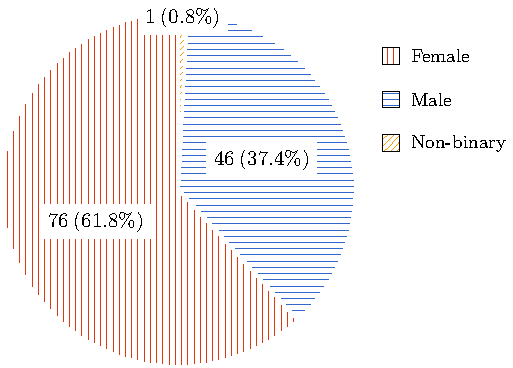
\includegraphics[width=9cm]{img/5-participants-sex.pdf}
  \end{center}
  \fonte{Author.}
\end{figure}

\begin{figure}[!htb]
  \caption{Participants Age Distribution}\label{fig:age-distribution}
  \begin{center}
    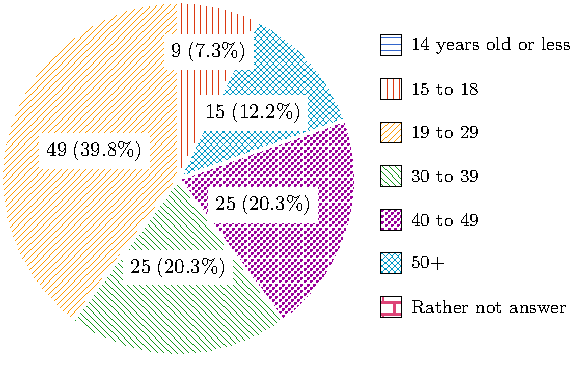
\includegraphics[width=.6\textwidth]{img/5-participants-age.pdf}
  \end{center}
  \fonte{Author.}
\end{figure}

\begin{figure}[!htb]
  \caption{Participants Formation Distribution}\label{fig:formation-distribution}
  \begin{center}
    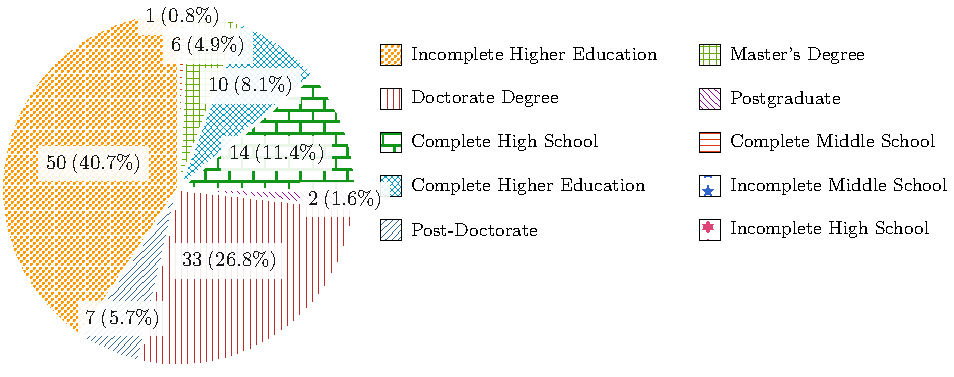
\includegraphics[width=\textwidth]{img/5-participants-formation.pdf}
  \end{center}
  \fonte{Author.}
\end{figure}

\begin{figure}[!htb]
  \caption{Community Roles Distribution}\label{fig:community-roles}
  \begin{center}
    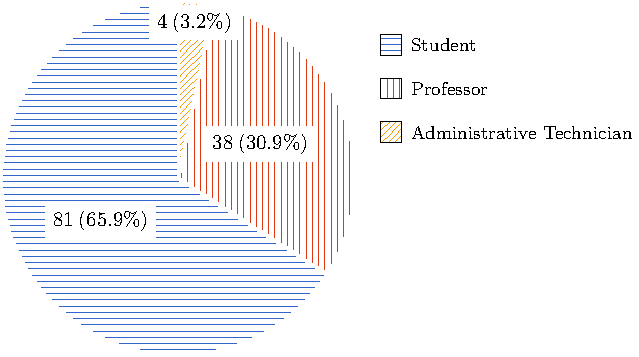
\includegraphics[width=11cm]{img/5-community-roles.pdf}
  \end{center}
  \fonte{Author.}
\end{figure}

\begin{figure}[!htb]
  \caption{Participants City Distribution}\label{fig:city-distribution}
  \begin{center}
    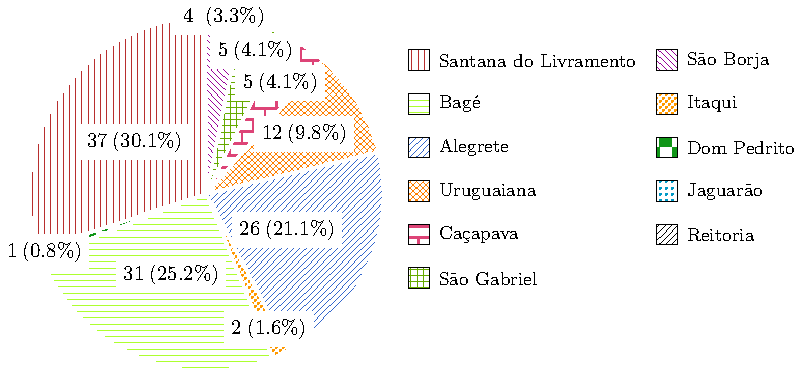
\includegraphics[width=.85\textwidth]{img/5-participants-city.pdf}
  \end{center}
  \fonte{Author.}
\end{figure}

\begin{figure}[!htb]
  \caption{Outreach Participation Distribution}\label{fig:outreach-participation}
  \begin{center}
    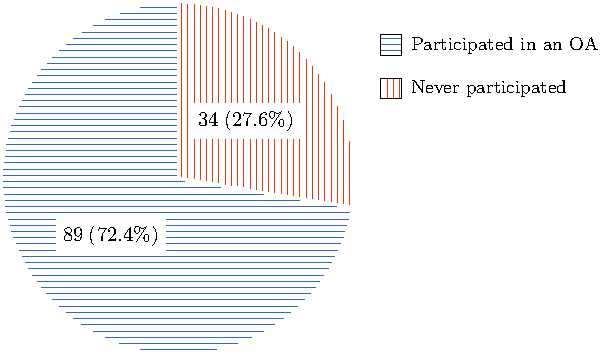
\includegraphics[width=.65\textwidth]{img/5-outreach-participation.pdf}
  \end{center}
  \fonte{Author.}
\end{figure}

\begin{figure}[!htb]
  \caption{Outreach Roles Distribution}\label{fig:outreach-roles}
  \begin{center}
    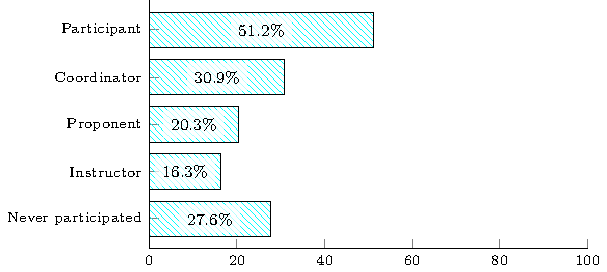
\includegraphics[width=13cm]{img/5-outreach-roles.pdf}
  \end{center}
  \fonte{Author.}
\end{figure}

\subsection{Quantitative Results}\label{sec:quantitative-results} % Participação em algum projeto de extensão

The MoSCoW scale, which was previously described, was used to ask respondents to prioritize the user story in the question in order to collect quantitative data.

By examining the responses to each of the questions in the questionnaire, which is available at \Cref{appendix:questionnaire}\footnote{As a note, to better navigate from the charts to the questions themselves, which are all the way down in the appendix, open the PDF in the browser and hit ``CTRL + F'', searching for the question \ac{ID} and using the arrows to navigate between occurrences.},some interesting results were found regarding each user role defined for the \ac{MVP}, which are going to be discussed later in more detail in \Cref{ext:roles}. The following sections describe the results obtained on each of their quantitative questions. The roles are as follows:
\begin{inparaenum}[(a)]
  \item Proponent,
  \item Coordinator,
  \item Instructor and
  \item Participant.
\end{inparaenum}

\subsubsection{Proponent} \label{sec:survey-quant-proponent}

Regarding the role of \ac{OA} proponent, the P(1-8) given written survey questions were appropriate, with the majority of them scoring Must haves and Should haves as shown in \Cref{fig:proponent-questions}, demonstrating the interest of end users, for the mentioned features. The only exceptions were P2 and P5, scoring the most of Could and Will not haves out of all of the questions.

In question P7, as can be seen in \Cref{fig:p7-question}, there was a sub question related to which communication channel the user would prefer for communicating with the future \ac{OA} participants. The respondents could check both alternatives, and it was unexpected that \textit{WhatsApp} got over half of votes, considering the history of using emails most of the time for communication in the university.

\begin{figure}[!htb]
  \caption{Questions Regarding Proponent Role}\label{fig:proponent-questions}
  \begin{center}
    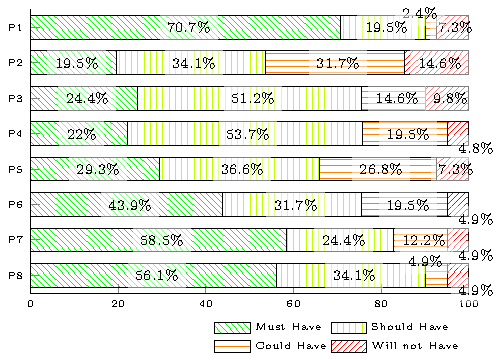
\includegraphics[width=13cm]{img/5-questions-proponent.pdf}
  \end{center}
  \fonte{Author.}
\end{figure}

\begin{figure}[!htb]
  \caption{Which communication channel the proponent prefers}\label{fig:p7-question}
  \begin{center}
    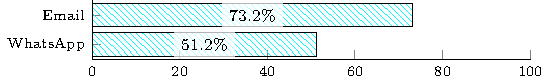
\includegraphics[width=.8\textwidth]{img/5-questions-proponent-P7-1.pdf}
  \end{center}
  \fonte{Author.}
\end{figure}

\subsubsection{Coordinator} \label{sec:survey-quant-coordinator}

For the role of coordinator, only two questions were asked to the respondents. Since it was assumed that the review and approval process of the \acp{OA} was as important as, if not more important than issuing participation certificates, it was interesting to see that the first question, C1, did not receive as many Must haves as C2. The results can be seen in \Cref{fig:coordinator-questions}.

\begin{figure}[!htb]
  \caption{Questions Regarding Coordinator Role}\label{fig:coordinator-questions}
  \begin{center}
    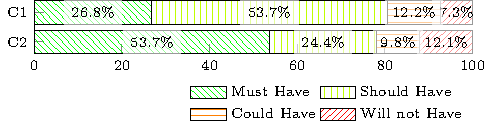
\includegraphics[width=.7\textwidth]{img/5-questions-coordinator.pdf}
  \end{center}
  \fonte{Author.}
\end{figure}

\subsubsection{Instructor} \label{sec:survey-quant-instructor}
As was previously noted, the survey respondents place a high value on the distribution of participation certificates. The only question relating to the Instructor role, which is illustrated in \Cref{fig:instructor-questions}, can be said to be similar because it is one of the user stories in the study with the highest priority, with over 60\% Must haves.

\begin{figure}[!htb]
  \caption{Questions Regarding Instructor Role}\label{fig:instructor-questions}
  \begin{center}
    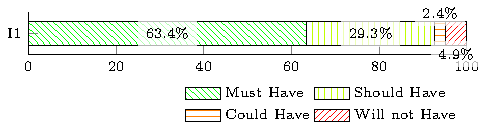
\includegraphics[width=.7\textwidth]{img/5-questions-instructor.pdf}
  \end{center}
  \fonte{Author.}
\end{figure}

\subsubsection{Participant} \label{sec:survey-quant-participant}

This user role is where most of the demographics for this survey are located. In order to achieve a balanced distribution of questions, all of the students were asked to respond only to the participant system user role, composed by 14 (fourteen) questions, while the teachers and \ac{ATE} provided responses for three different profiles, which together totaled 11 (eleven) questions composed by. 

The questions were split between two graphs, the first half being on \Cref{fig:participant-1}, and the second half being on \Cref{fig:participant-2}. Most of the user stories present in these questions received high Must haves scores, demonstrating the importance of the requirements raised. However, not all of them were ranked highly, such as A11 and A13, which showed an above average number for Could and Will not haves.

It makes sense that respondents attribute these ratings to A11, as the question relates to the point of view of someone outside the academic community. This user story is also a little bit of out scope for an \ac{MVP}, so the feedback was important to rank it lower in the requirements.

A13 was thought up during meetings with the advisor, and it seemed to be a very good feature, but in the view of the respondents it was not, exemplifying the importance of carrying out a survey with end users.

Last but not least, A14 included a sub-question, seen in \Cref{fig:participant-A14}, that was similar to P7 and asked respondents to select the location where they would prefer to view the upcoming \acp{OA} they were enrolled in. It was great to know ahead of time that most users would prefer to export the \ac{OA} to their own calendar apps rather than adding a calendar view to the website itself.

\begin{figure}[!htb]
  \caption{Questions Regarding Participant Pt.1}\label{fig:participant-1}
  \begin{center}
    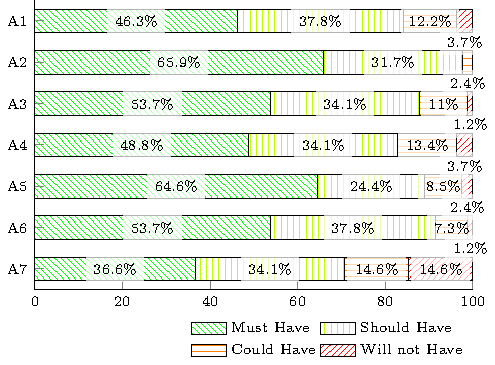
\includegraphics[width=.7\textwidth]{img/5-questions-participant-1.pdf}
  \end{center}
  \fonte{Author.}
\end{figure}

\begin{figure}[!htb]
  \caption{Questions Regarding Participant Pt.2}\label{fig:participant-2}
  \begin{center}
    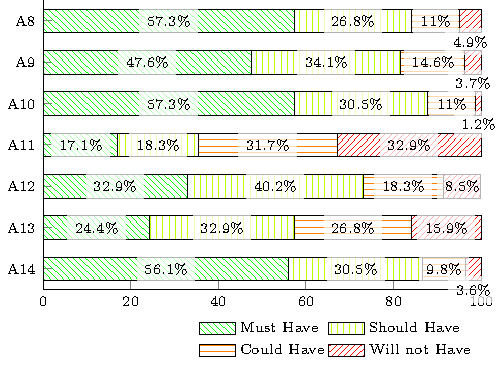
\includegraphics[width=.7\textwidth]{img/5-questions-participant-2.pdf}
  \end{center}
  \fonte{Author.}
\end{figure}

\begin{figure}[!htb]
  \caption{Where the user would rather see their upcoming \ac{OA}} \label{fig:participant-A14}
  \begin{center}
    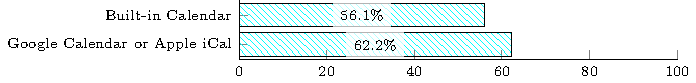
\includegraphics[width=\textwidth]{img/5-questions-participant-A14-1.pdf}
  \end{center}
  \fonte{Author.}
\end{figure}

\subsection{Qualitative Results} \label{sec:qualitative-results}% Classificação final, graficos
% =========================
% Para as respostas coletadas nas perguntas open-ended, em que foram apontadas melhorias e sugestões para os pesquisadores, algumas entre elas se destacaram pelo seu valor de importancia para alcancar o objetivo do estudo. Dentre os dois grupos de respostas, discentes e docentes/TAE, o segundo grupo gerou resultados mais robustos e com mais propriedade, justamente pelo motivo de ja experienciarem estas atividades burocraticas em seu dia a dia.

For the answers collected in the open-ended questions, in which improvements and suggestions for the researchers were pointed out, some among them stood out for their importance value to achieve the objective of the study. Among the two groups of responses, the first one being composed by students and the second by teachers and \acp{ATE}, the second group generated more robust and more appropriate results, precisely because they already experience these bureaucratic activities in their daily lives.
% ==========================

The responses will be translated freely from their original language, Portuguese and some of the most relevant answers given by respondents in the first group are mentioned below, they highlight improvements in the structure of the questionnaire together with suggestions for functionalities, they are:
\begin{itemize}
  \item  ``\textit{Regarding A9, it would be cool to send out notifications, for instance, when an \ac{OA}'s registration deadline is approaching}''. This was a very interesting and valid suggestion, which, besides the notifications part, opens doors to features such as having an \ac{OA} watchlist and saving favorites;
  \item ``\textit{The questions are repetitive, leading the individual to declare them irrelevant}''. This was unexpected input on the survey's questions because it wasn't raised at any point during the survey's development. Nevertheless, it was excellent feedback;
  \item ``\textit{Change the order of importance and the highest level of satisfaction since the order of presentation of the points was incorrect at the beginning of the question because it starts with number 4}''. Maybe setting the MoSCoW scale in reverse, starting as Must Have as a 1, instead of a 4, would add more value. However, this was the only criticism written on this topic.
\end{itemize}

The ideas raised by the respondents of the second group are presented and discussed below:
\begin{itemize}
% ====================================
% \item Dois respondentes deste grupo levantaram a questão que se refere ao retrabalho e quantidade de informações a serem preenchidas. Eles ressaltam que por hoje as atividades de extensão terem que ser cadastradas no projeto SAP, é de grande importncia que a ferramenta final consiga gerar um relatório no modelo aceito por esta ferramenta, caso isto não seja cumprido, apenas geraria mais trabalho para os docentes tendo que preencher em ambas as ferramentas. Um deles também atenta que para ele seria muito mais interessante que os formulários na ferramenta sejam o maximo sucintos, facilitando o preenchimento e não adicionando tanta carga burocratica extra.

\item Two respondents from this group raised the question regarding rework and the amount of information to be filled in. They point out that for today the \aclp{OA} will have to be registered in the \ac{SAP} project, it is of great importance that the final tool manages to generate a report in the model accepted by this tool, if this is not fulfilled, it would only generate more work for the professors having to fill in both tools. One of them also notes that it would be much more interesting for him if the forms in the tool were as succinct as possible, making it easier to fill in and not adding so much extra bureaucratic burden;
% ====================================

% ====================================
% \item Outro ponto muito bem lembrado por outro respondente deste grupo, se refere a participantes que tem historicos de desistencias ou baixa participaç~ao em atividades em que são inscritos, fazendo o mal uso de sua vaga. Para solucionar isso foi sugerido que o sistema tenha conhecimento destes individuos e no momento em que ele fora colocado em uma fila de inscrição de uma atividade, este tenha menos prioridade do que alguém que é assíduo com seus compromissos.

\item Another point that was very well remembered by another respondent in this group refers to participants who have a history of dropouts or low participation in activities in which they are enrolled, making misuse of their vacancy. To solve this, it was suggested that the system be aware of these individuals and at the time they were placed in an activity registration queue, they would have less priority than someone who is assiduous with their commitments;
% ====================================

% ====================================
% \item Uma dor levantada por um coordenador de atividades de extensão, diz a respeito das gerações de certificados que fica responsável pela PROEXT, mas na maioria das vezes o progresso de geração e prazo estimado não são informados para o coordenador encarregado. Por este motivo, os participantes, que não sabem como funciona este processo, ficam perguntando diretamente para o coordenador e não para a própria PROEXT, causando-o incomodo. Este sugere que haja alguma maneira em que possa ser deferida notificações, ou até mesmo um recurso de visualização informando a data prevista para a geração dos certificados.

\item A pain raised by an outreach activities coordinator, says about the generations of certificates that \ac{PROEXT} is responsible for, but most of the time the generation progress and estimated time are not reported to the coordinator in charge. For this reason, the participants, who do not know how this process works, keep asking the coordinator directly and not to \ac{PROEXT} itself, causing them discomfort. This suggests that there is some way in which notifications can be deferred, or even a visualization feature informing the expected date for the generation of certificates;
% ====================================

% ====================================
% \item A geração de certificados é um processo indispensavel no ciclo de vida de uma atividade de extensão, logo este processo deve ser o menos cansativo possível, mas isto não acontece, de acordo com um respondente do segundo grupo, ele diz que hoje em dia a geraç~ão dos certificados é feita um por um no sistema SEI, e este processo é bastante lento. Ele sugere que este processo seja o mais simples possível permitindo a geração de todos os certificados de uma só vez.

\item The generation of certificates is an indispensable process in the life cycle of an \acl{OA}, so this process should be as tiring as possible, but this does not happen, according to a respondent from the second group, he says that nowadays the generation of of certificates is done one by one in the \ac{SEI} system, and this process is quite slow. He suggests that this process be as simple as possible, allowing the generation of all certificates at once;
% ====================================

% ====================================
% \item Relacionado ao tópico anterior de certificados, outro respondente afirma que seria interessante, principalmente para o público externo, a possibilidade de geração de certificado sem ter que esperar pela data de finalizaç~ão do projeto, informando que o participante esta devidamente matriculado na atividade.

\item Related to the previous topic of certificates, another respondent states that it would be interesting, especially for the external public, to be able to generate a certificate without having to wait for the project completion date, informing that the participant is duly enrolled in the activity.
% ====================================
\end{itemize}

\section{Chapter Summary}

The survey as a whole was covered in this chapter, including information regarding the protocol that was followed, the methods used to generate the questions, threats to validity, and both a quantitative and qualitative analysis of the outcomes. \Cref{extensionly} will go into further detail on the particulars of the Backend MVP that will be produced, discussing architecture choices, DevOps processes, tools and other topics.
